\documentclass[12pt, onecolumn]{article}


\usepackage[utf8]{inputenc}
\usepackage[italian]{babel}

\usepackage{graphicx}
\usepackage{enumitem}

%opening
\title{Time Series Final Project}
\author{Pranav Kasela \\$846965$}
\date{}
\begin{document}

\maketitle

\section*{Introduzione}
Lo scopo del progetto è studiare una serie temporale riguardante dati dell'elettricità, facendo una previsione sul suo andamento nei 11 mesi dell'anno successivo, per cui verranno utilizzate tre metodologie diverse: ARIMA, UCM e reti neurali ricorsive.\\
Per confrontare tale metodologie verrà utilizzata la metrica MAPE e confronto visivo, poiché un modello potrebbe fare una predizione costante e ottenere un MAPE comunque basso.
\begin{figure}[!h]
  \centering
  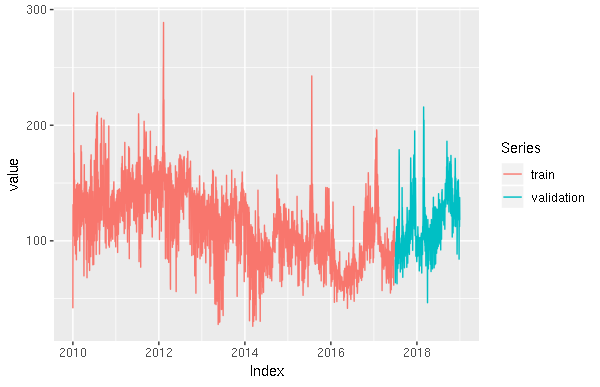
\includegraphics[width=\linewidth, height=7cm]{imgs/Series.png}
  \caption{Grafico della Serie}
  \label{fig:series}
\end{figure}\\
Per l'allenamento dei modelli l'ultimo anno e mezzo dei dati viene tenuto separato (Figura \ref{fig:series}), esso fungerà da validation set sul quale verranno confrontati le varie metodologie di previsione.
Come metrica comune alle varie metodologie è stata scelta MAPE perché più facile da capire da un punto di vista umano, si poteva benissimo scegliere anche la MSE o la MAE che sarebbero perfetti per un confronto tra metodologie, ma non spiegherebbero come un modello in particolare performa relativamente ai dati.
Mentre per il confronto nelle metodologie stesse, i.e., modelli con diversi iper-parametri o architetture si sceglieranno delle metriche diverse, e verranno dette quando si spiega ciascun modello.\\
Nella serie si notano alcuni picchi particolarmente alti, non vengono trattati poiché non si sa l'origine della serie e potrebbero potenzialmente essere dei picchi che contengono qualche informazione particolare (qualche evento anomalo) oppure potrebbero aver influenzato tutta la serie, infatti si nota che la serie cambia il suo trend subito dopo questi picchi (potrebbe anche essere solo una coincidenza).
\section*{ARIMA}
Si usa la classe xts per definire la serie temporale (xts perché la serie è giornaliera nei vari anni), plottando ACF e PACF (Figura \ref{fig:ACF_1}) si vede immediatamente l'esistenza di tutte tre componenti stagionali con stagionalità 7: AR$(1)_7$I$(1)_7$MA$(1)_7$ poiché si vede una discesa geometrica (ogni 7 giorni) nel grafico della PACF e una discesa lineare (ogni 7 giorni) nel grafico della ACF, l'esistenza della parte di integrazione stagionale si può vedere anche facendo un modello SARMA$(1,1)_7$ e vedendo che il coefficiente di SAR risulta essere molto vicino ad 1. 
\begin{figure}[!h]
  \centering
  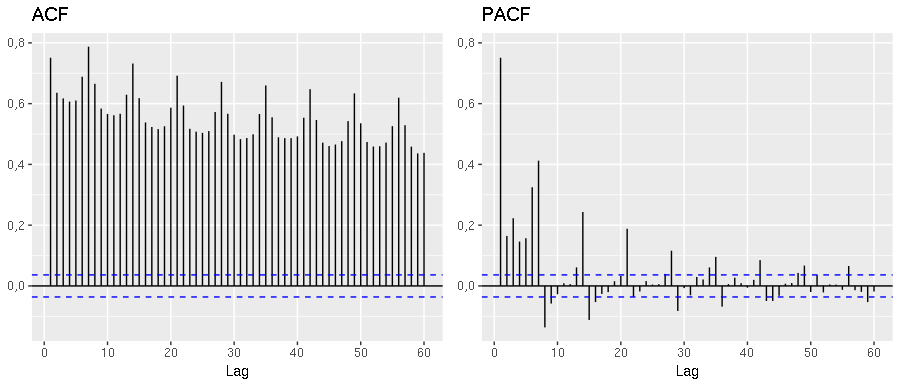
\includegraphics[width=\linewidth,height=4cm]{imgs/ACF_1.png}
  \caption{ACF e PACF della Serie.}
  \label{fig:ACF_1}
\end{figure}\\
Vi sembra essere anche quale componente non stagionale oltre ad una possibile parte di integrazione dovuta all'esistenza di qualche trend nella serie, ciò viene studiato sui residui dopo aver applicato il modello SARIMA$(1,1,1)_7$.
Sui grafici della ACF/PACF dei residui (Figura \ref{fig:ACF_2}) si vede che c'è un modello ARMA ma non si riesce a capire facilmente quali siano i coefficienti.\\
Per questa ragione si effettua una Grid Search con i coefficienti (potenze del polinomio caratteristico) di AR e MA che variano da 0 a 6 mentre teniamo fissi la parte stagionale SAR$(1,1,1)_7$, e scegliamo il modello con la log-likelihood più alta: Il modello con la log-likelihood più alta risulta essere un ARMA(6,6). Calcolando i moduli delle radici del polinomio AR del modello ARIMA$(6,0,6)(1,1,1)_7$ si vede che sono molto vicini ad 1, ciò significa che la serie aveva, come già si sospettava,  una parte di integrazione, si prova con la prima integrazione e questo problema viene risolto, quindi il modello finale proposto è un ARIMA$(6,1,6)(1,1,1)_7$. Gli ACF/PACF dei residui dell'ultimo modello proposto sono per la maggior parte rientrati nelle bande, quei pochi che escono fuori hanno valori molto bassi. \\
\begin{figure}[!h]
  \centering
  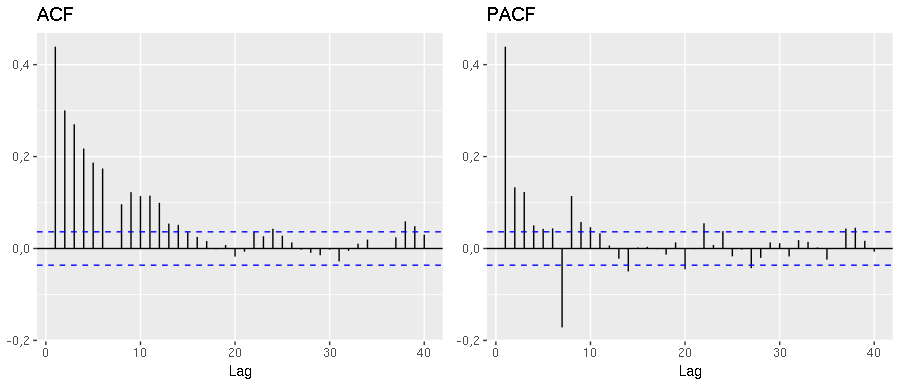
\includegraphics[width=\linewidth,height=5cm]{imgs/ACF_2.png}
  \caption{ACF e PACF dei residui del primo modello.}
  \label{fig:ACF_2}
\end{figure}
\begin{figure}[!h]
  \centering
  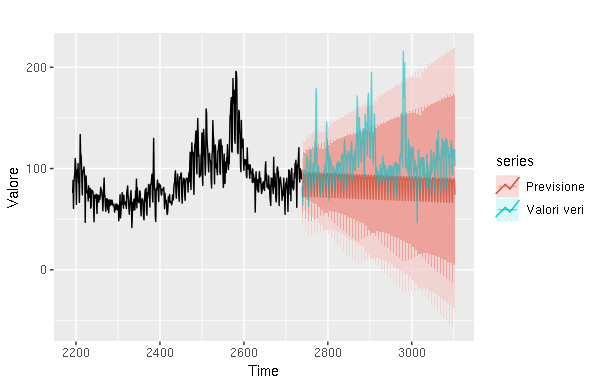
\includegraphics[width=\linewidth,height=6cm]{imgs/forecast_ar_1.png}
  \caption{Previsione della Serie sul Validation.}
  \label{fig:ARIMA_pred}
\end{figure}\\
Dalle previsioni di questo modello, mostrate nella Figura \ref{fig:ARIMA_pred}, si capisce immediatamente che queste componenti non spiegano tutta la varianza del modello, infatti questa serie è una serie multi stagionale, R non permette di trattare ARIMA multi stagionale quindi si introducono dei regressori esterni.\\
Per risolvere il problema di multi stagionalità si usano 24 regressori sinusoidali con frequenza base annua, il numero 24 è stato calcolato usando il validation set.
In questo modo il MAPE sul validation è $14.50\%$.\\
Si aggiungono altri regressori esterni: i giorni festivi, dando più importanza alle festività più importanti come il natale, pasqua, ferragosto e il nuovo anno e raggruppando le altre festività in un'unica variabile, il MAPE in questo caso aumenta arrivando al $18.03\%$.
Si opta per il primo modello che non usa regressori per le vacanze visto che ottiene un MAPE più basso sul validation.
\begin{figure}[!h]
  \centering
  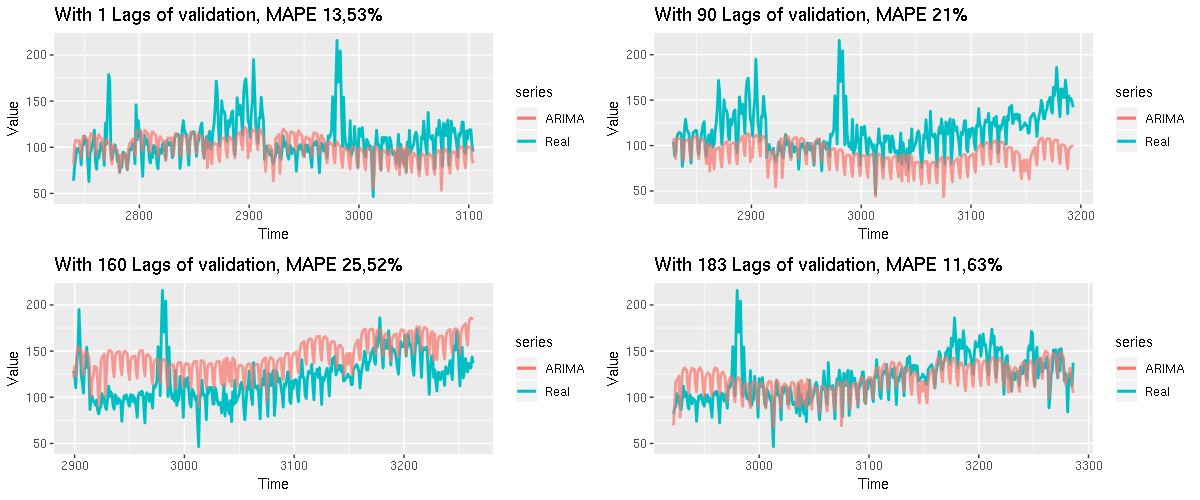
\includegraphics[width=\linewidth,height=6cm]{imgs/forecast_arima.png}
  \caption{Previsione su alcuni elementi del validation usando XARIMA.}
  \label{fig:XARIMA_pred}
\end{figure}\\
Nella figura \ref{fig:XARIMA_pred} si vede subito i regressori trigonometrici annua spiegano molta varianza del modello.\\
Nel modello finale con regressori trigonometrici se si provano a vedere i residui si vede che qualche picco sul ACF e PACF esce fuori (anche se di poco) dagli intervalli, e anche il test di Ljung-Box non rifiuta l'ipotesi nulla di non autocorrelazione al $95\%$, quindi i residui non sono un WN, ma in una serie con dati reali è molto difficile arrivare a residui che sono perfettamente un WN, un cosa che può notare è che i residui sono distribuiti abbastanza come un normale con media 0 (Figura \ref{fig:res}).
\begin{figure}[!h]
  \centering
  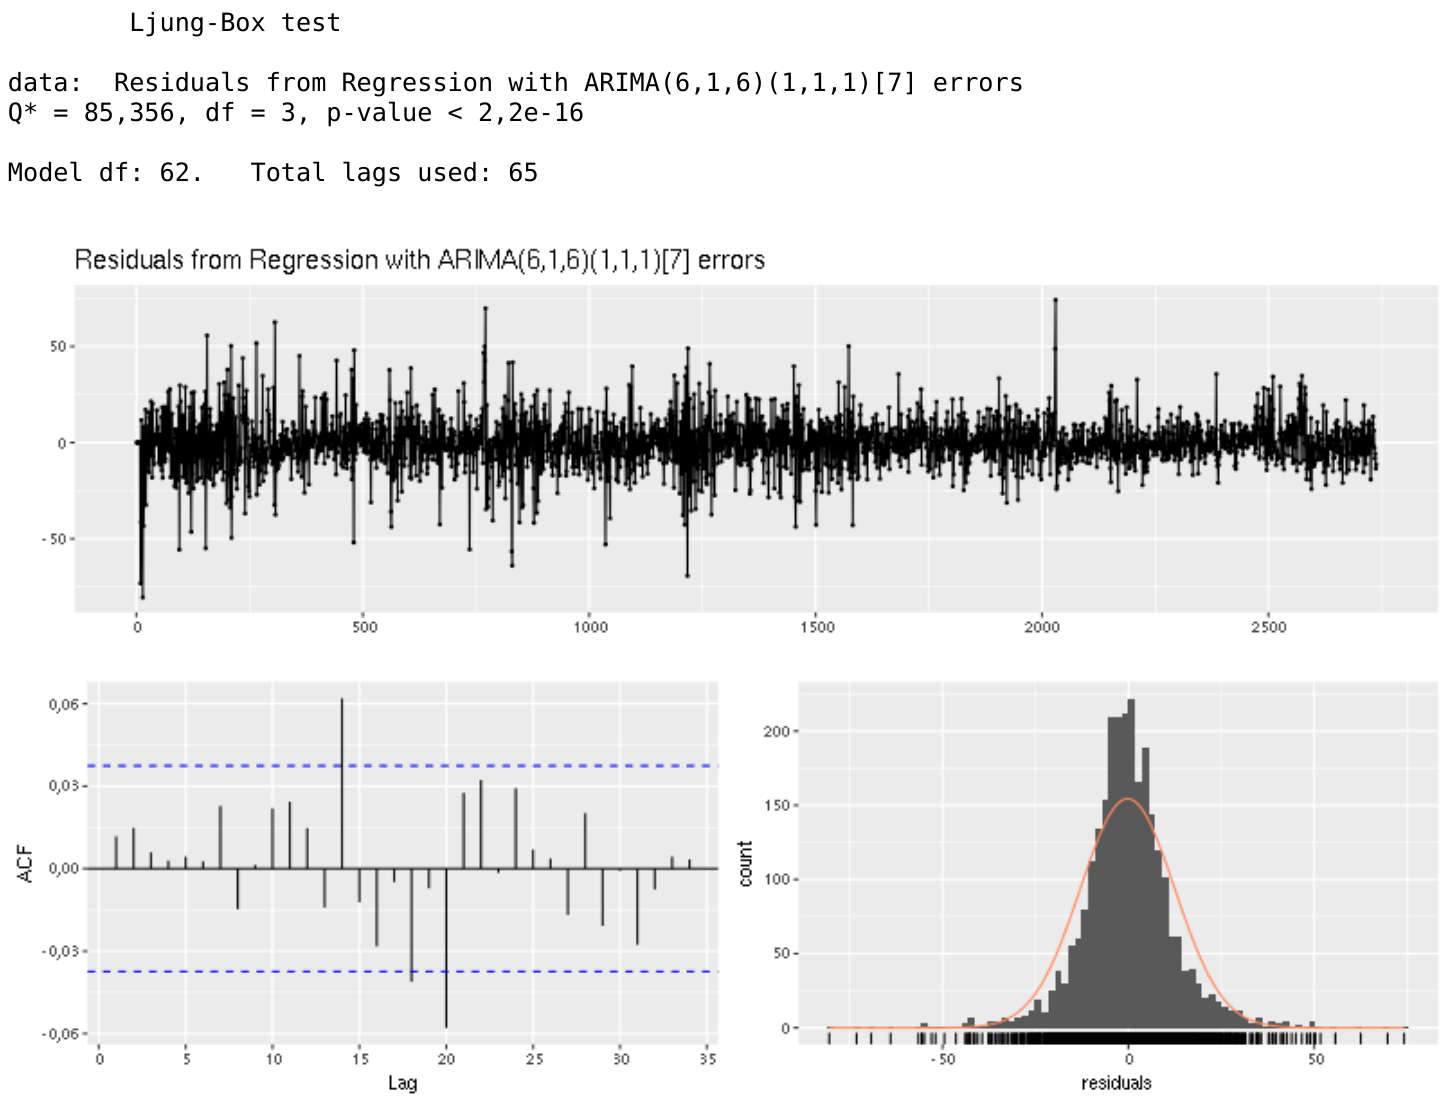
\includegraphics[width=\linewidth,height=6cm]{imgs/arima_res.png}
  \caption{Residui del modello ARIMA.}
  \label{fig:res}
\end{figure}
\section*{UCM}
Usando le considerazioni fatte per l'ARIMA si usa un modello UCM con un local linear trend, una componente stagionale settimanale stocastica con dummy e una componente stagionale stocastica annua con 24 regressori trigonometrici.
Si provano due modelli: il primo usando i regressori per le vacanze costruite per l'ARIMA e il secondo senza l'ausilio di questi regressori.
Per la validazione del modello si usa il predict di SSModel, che a sua volta sfrutta KFS e gestisce in automatico le modifiche necessarie alle strutture SSModel per effettuare delle previsioni come si vede dal codice sorgente\footnote{https://github.com/cran/KFAS/blob/master/R/predict.SSModel.R}, quindi in questo modo è più facile introdurre nuovi dati nel modello senza dover rivalutare i parametri del modello state space.\\
Per il predict di SSModel bisogna passare il modello fittato usando i dati di train e un altro modello sempre della classe SSModel con gli stessi parametri ma con dati del validation seguiti da NA laddove bisogna fare predire al modello usando l'algoritmo di Kalman.\\
Il modello senza regressori ottiene un MAPE più basso rispetto al modello con i regressori, quindi si opta per usare il modello UCM senza i regressori.
Questo è un comportamento analogo ai modelli ARIMA, ciò significa che questi regressori per le vacanze non aiutano a spiegare i dati.\\
Il MAPE sul validation del modello con regressori è $22.01\%$ mentre del modello senza regressori è $18.94\%$.
Si tentano altri due modelli UCM senza regressori, uno usando RW integrato e l'altro solo con RW: il primo ottiene un MAPE di $16.76\%$sul validation mentre il secondo ottiene un MAPE di $18.09\%$.
Viene quindi scelto modello senza regressori con un RW integrato.
Nella Figura \ref{fig:UCM_pred} sono presente alcune stime effettuate sui dati del validation con i relativi errori.
\begin{figure}[!h]
  \centering
  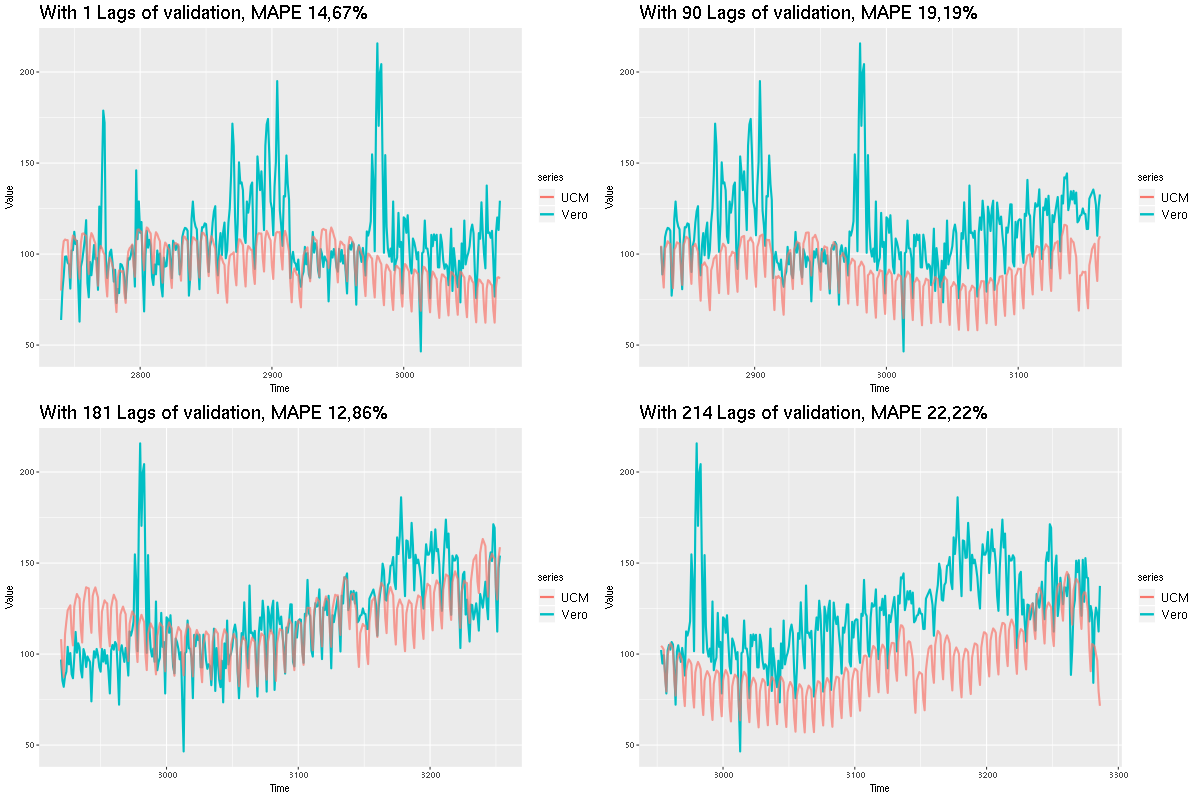
\includegraphics[width=\linewidth,height=5.5cm]{imgs/forecast_ucm.png}
  \caption{Previsione su alcuni elementi del validation usando UCM.}
  \label{fig:UCM_pred}
\end{figure}
\section*{LSTM}
Come ultimo modello è stato usato una rete neurale con nodi LSTM, sono stati testati anche le alternative come GRU o le più semplici RNN senza avere dei risultati migliori rispetto allo LSTM (le GRU avevano prestazioni molto simili alle LSTM).\\
Il train e validation è lo stesso usato per ARIMA e UCM in modo da poterli confrontare.
I dati vengono standardizzati per avere media 0 e varianza 1, dove la standardizzazione si ottiene dal training set.\\
I dati vengono modificati per avere una struttura più adatta per il machine learning in generale, quindi si fissa L'INPUT\_SIZE che rappresenta quanti istanti temporali può guardare indietro il modello per prevedere n istanti successivi indicati con OUTPUT\_SIZE.
In questo caso OUTPUT\_SIZE è 334 visto che l'obiettivo è prevedere dal 2019-01-01 al 2019-11-30 che sono 334 giorni, mentre INPUT\_SIZE è 730 giorni (due anni) che è un buon compromesso tra avere un numero di dati sufficiente per l'allenamento della rete neurale e un grado di informazione sufficiente per la previsione.\\
Allenare la rete per predire tutte le previsioni insieme è più efficace e riduce molto di più l'errore rispetto ad allenarlo per fare previsione un passo in avanti e usare la nuova predizione per fare ricorsivamente altre predizioni.\\
Sono state provate tre architetture:
\begin{itemize}[leftmargin=*]
\item Input$\to$LSTM(tanh)$\to$Dense(relu)$\to$Dense(relu)$\to$Output.
\item Input$\to$LSTM(tanh)$\to$Dense(relu)$\to$Dense(relu)$\to$Dense(relu)$\to$Output.
\item Input$\to$LSTM(tanh)$\to$LSTM(tanh)$\to$Dense(relu)$\to$Dense(relu)$\to$Output.
\end{itemize}
L'ottimizzatore di tutte e tre i modelli è RMSprop e la loss è `mse'. Gli iper-parametri di questo modello: il numero di unità LSTM, il numero di neuroni nei layer fully connected, il learning rate iniziale e il batch size, sono stati calcolati usando AutoML.
Inoltre nell'allenamento sono stati due callbacks di keras: uno per diminuire il learning rate in caso il modello non migliori sulla validation loss per almeno tre volte di seguito e uno per fermare l'allenamento nel caso il modello non migliori per oltre 50 epoche.
Il numero di epoche invece viene fissato a 100, che non è un numero ottimizzato ma compensato dall'esistenza dei callbacks.
Per AutoML è stato scelto come score la validation loss (mse) e come modello surrogato è stato scelto il GP con la EI come funzione di acquisizione, la libreria di python usata è sherpa-ai, che usa GPyOpt per l'ottimizzazione gaussiana, il numero di iterazioni è 100.\\
Come esempio nella Figura \ref{fig:automl} è indicato l'andamento dell'ottimizzazione utilizzando GP per la prima architettura.
\begin{figure}[!h]
  \centering
  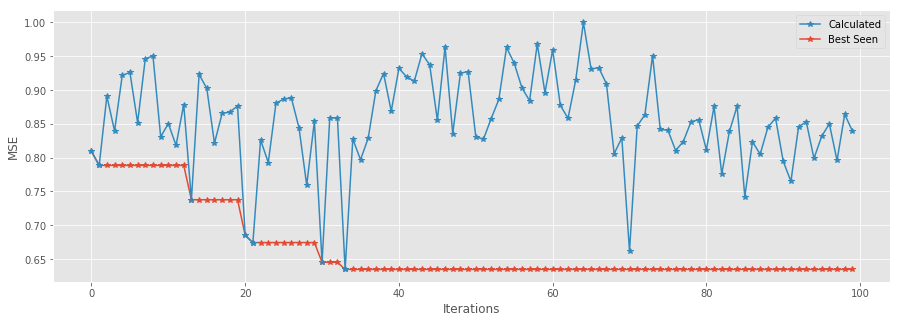
\includegraphics[width=\linewidth,height=4cm]{imgs/automl_1.png}
  \caption{Risultati del AutoML.}
  \label{fig:automl}
\end{figure}\\
Il miglior modello delle tre architettura dopo AutoML ottiene i seguenti MAPE sul validation:
\begin{enumerate}[noitemsep, topsep=0ex]
\item Primo: $15.93\%$
\item Secondo: $15.75\%$
\item Terzo: $15.89\%$
\end{enumerate}
Il miglior modello è il secondo, nella Figura \ref{fig:LSTM_pred} vengono mostrate le sue previsioni per gli stessi validation del ARIMA e UCM. Visto che la differenza tra i MAPE dei modelli è bassa non sono state provate altre architetture.
\begin{figure}[!h]
  \centering
  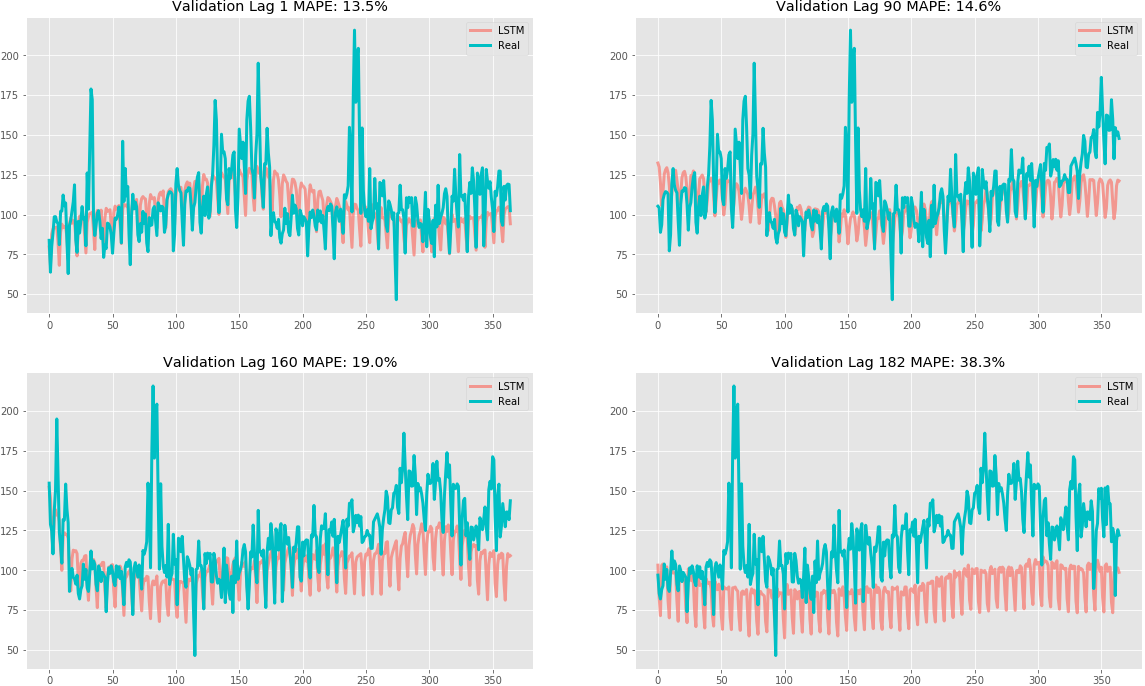
\includegraphics[width=\linewidth,height=6cm]{imgs/forecast_lstm.png}
  \caption{Previsione su alcuni elementi del validation usando LSTM.}
  \label{fig:LSTM_pred}
\end{figure}\\
Nei modelli LSTM non è possibile usare direttamente regressori esterni (se non introdotti come una serie che farebbero riferimento a qualcosa nel passato), un modo per provare a inserire regressori esterni è creare un altro layer di input con questi regressori e concatenarli al modello dopo i layer LSTM, ma se si prova a fare una predizione 334 passi avanti, aumentano il numero dei neuroni e delle connessioni e quindi aumenta anche il numero dei dati richiesti per l'allenamento, inoltre visto che non hanno dato informazioni aggiuntive (anzi hanno solo peggiorato le performance) nei modelli ARIMA e UCM, è stato reputato inutile provare ad aggiungere questi regressori al modello.
\section*{Conclusioni}
I risultati delle tre metodologie sono:
\begin{table}[!h]
  \centering
  \begin{tabular}{|l|c|c|c|}
    \hline
    Model & ARIMA & UCM & LSTM\\
    \hline
    Training & $9.50\%$ & $10.98\%$ & $13.65\%$\\
    Validation & $14.50\%$ & $16.76\%$ & $15.75\%$\\
    \hline
  \end{tabular}
  \caption{Confronto dei risultati ottenuti dalle tre metodologie }
  \label{tab:confronto}
\end{table}\\
Le performance delle varie metodologie non sono molto diverse tra di solo, quindi colgono più o meno le stesse informazioni dai dati, il modello che riesce a tirar fuori più informazioni è l'ARIMA, seguito dal modello LSTM.\\
Per le previsioni sul test i dati del train e validation vengono riuniti e si ri-allenano i modelli utilizzando i dati totali, per il modello della rete neurale il modello viene semplicemente allenato per altre 100 epoche sui dati del validation, per dare un po' di peso in più ai dati del validation che sono più recenti.\\
Si nota che nelle previsioni sul test set, raffigurate nella Figura \ref{fig:test_pred}, le previsioni di UCM e ARIMA sono molto simili ma la rete LSTM tende a ritardare la discesa dei prezzi, quindi si crede che nel testing la rete LSTM avrà performance anche molto diverse rispetto ai due modelli lineari: Negli ultimi anni l'andamento dei prezzi è diverso, i modelli lineari riescono quindi ad adattarsi velocemente ai nuovi dati mentre nell'allenamento la rete LSTM non fa differenza tra i dati vecchi o nuovi e cerca di minimizzare l'errore sulla serie globale quindi il nuovo andamento dipende in egual misura sia da dati recenti che dati vecchi da cui si spiega l'andamento diverso del modello LSTM dai modelli ARIMA e UCM.
\begin{figure}[!h]
  \centering
  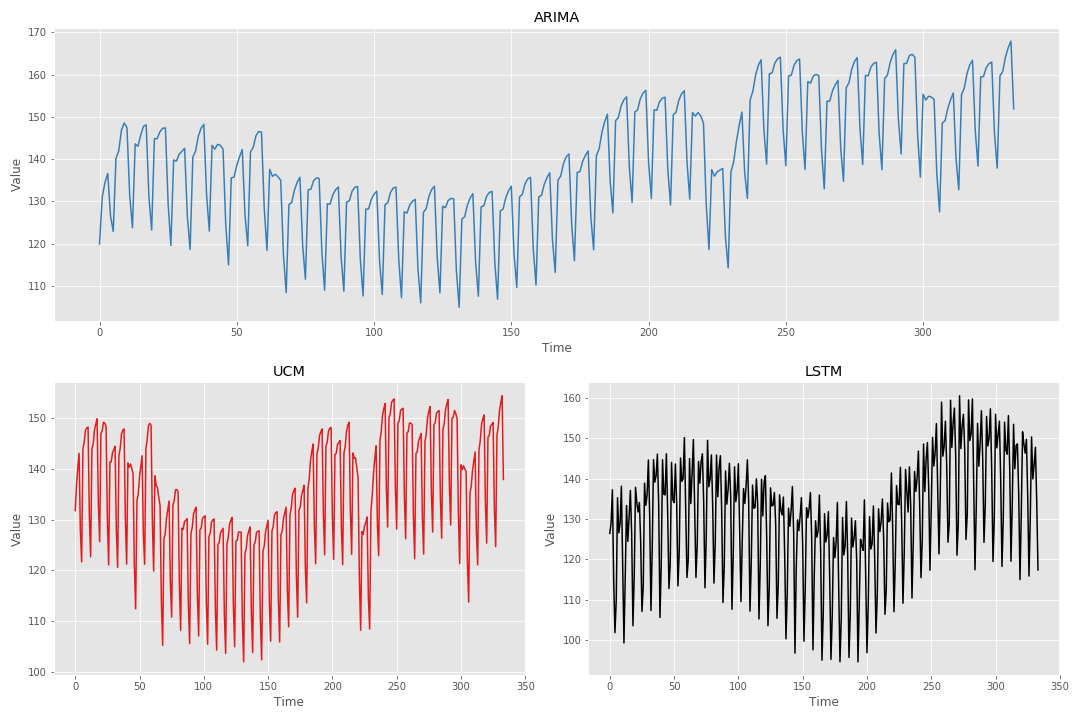
\includegraphics[width=\linewidth,height=8cm]{imgs/test_results.png}
  \caption{Previsioni finali per il test.}
  \label{fig:test_pred}
\end{figure}\\
La `facilità' dei modelli come le reti neurali è che essi riescono a cogliere la maggior parte delle varie stagionalità e trend da soli se il numero di dati è sufficientemente grande, ad esempio nel caso di studio le stagionalità e il trend vengono colte molto bene, il modello LSTM mentre nei modello lineari classici bisogna studiare la serie `a mano' e aggiustare le componenti del modello.\\
Un modo per poter sfruttare la potenza di entrambi potrebbe essere quello di studiare un modello lineare classico prima e usare un modello RNN sui residui del primo modello, in modo da lasciar apprendere alla RNN ciò che non si è riusciti a spiegare nel modello classico (ammesso che ci sia qualcosa ancora da spiegare) oppure il viceversa.
Si possono usare altri modelli per lo studio dei residui come i modelli GARCH (per spiegare le varianze) che in questo caso potrebbe essere più utile visto che il test di Ljung-Box ha rigettato l'$H_0$ della non dipendenza dei residui e la varianza degli errori sembra oscillare nel tempo (e il logaritmo non riesce a schiaccarla).\\
Provando ad usare una rete LSTM in questo caso sui residui del modello ARIMA, in realtà, prevede valori talmente bassi da poter essere considerati tutto trascurabili, cioè il modello non riesce a tirar fuori nessuna informazione aggiuntiva significativa.


\end{document}